\documentclass[handout]{beamer}

\usetheme[progressbar=frametitle]{metropolis}
\usepackage{appendixnumberbeamer}
\usepackage{booktabs}
\usepackage{amsmath}
\usepackage{amssymb}
\usepackage{tcolorbox}
\usepackage{tikz}
\usetikzlibrary{patterns}
\definecolor{mycolor}{HTML}{DAE8FC}
\definecolor{mycolor2}{HTML}{EDDAFC}
\definecolor{mycolor3}{HTML}{FFBE97}
\definecolor{metropolisblue}{RGB}{39, 59, 94}



% Begin document
\begin{document}

% Title page
\title{Neural Network Variants}
\author{Zeel B Patel, Nipun Batra}
\date{\today}
\institute{IIT Gandhinagar}
\maketitle

\begin{frame}{Notation}
    \begin{table}
        \centering
        \begin{tabular*}{\textwidth}{@{\extracolsep{\fill}}ll}
            \toprule
            Symbol & Meaning \\
            \midrule
            
\begin{tikzpicture}
                \node[draw, circle, fill=metropolisblue, text=white] (x1) at (0, 0) {};
            \end{tikzpicture} & Input node \\
            
\begin{tikzpicture}
                \node[draw, circle, fill=none, text=black] (n11) at (1, 0) {};
            \end{tikzpicture} & Trainable parameter \\
            
\begin{tikzpicture}
                \node[draw, circle, pattern=north east lines, text=black] (n12) at (2, 0) {};
            \end{tikzpicture} & Non-trainable parameter \\
            % show forward pass nodes
            \bottomrule

        \end{tabular*}
    \end{table}

\end{frame}

\begin{frame}{Homoscedastic model with fixed noise}
    % partition page into two columns
    \begin{columns}[T,onlytextwidth]
        \column{0.6\textwidth}
        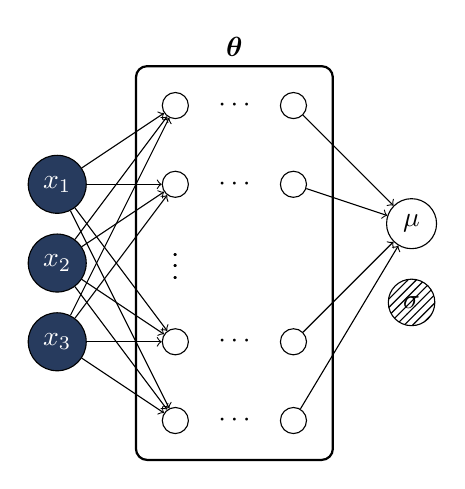
\begin{tikzpicture}
            \pgfmathsetmacro{\firstCol}{0}
            \pgfmathsetmacro{\secondCol}{1.5}
            \pgfmathsetmacro{\thirdCol}{3}
            \pgfmathsetmacro{\fourthCol}{4.5}

            \node[draw, circle, fill=metropolisblue, text=white] (x1) at (\firstCol, 1) {$x_1$};
            \node[draw, circle, fill=metropolisblue, text=white] (x2) at (\firstCol, 0) {$x_2$};
            \node[draw, circle, fill=metropolisblue, text=white] (x3) at (\firstCol, -1) {$x_3$};

            \node[draw, circle, fill=none, text=black] (n11) at (\secondCol, 2) {};
            \node[draw, circle, fill=none, text=black] (n12) at (\secondCol, 1) {};
            \node[draw, circle, fill=none, text=black] (n13) at (\secondCol, -1) {};
            \node[above=0.5cm] at (n13.north) {$\vdots$};
            \node[draw, circle, fill=none, text=black] (n14) at (\secondCol, -2) {};

            % connect all x to all n1 with a for loop
            \foreach \i in {1, 2, 3}
            \foreach \j in {1, 2, 3, 4}
            \draw[->] (x\i) -- (n1\j);

            % create a layer with all horizontal dots
            \foreach \i in {1, 2, 3, 4}
            \node[right=0.25cm] at (n1\i.east) {$\cdots$};

            % create next layer
            \node[draw, circle, fill=none, text=black] (n21) at (\thirdCol, 2) {};
            \node[draw, circle, fill=none, text=black] (n22) at (\thirdCol, 1) {};
            \node[draw, circle, fill=none, text=black] (n23) at (\thirdCol, -1) {};
            \node[above=0.5cm] at (n13.north) {$\vdots$};
            \node[draw, circle, fill=none, text=black] (n24) at (\thirdCol, -2) {};

            % create next layer
            \node[draw, circle, fill=none, text=black] (n31) at (\fourthCol, 0.5) {$\mu$};
            \node[draw, circle, pattern=north east lines, text=black] (n32) at (\fourthCol, -0.5) {$\sigma$};

            % connect all n1 to all n2 with a for loop
            \foreach \i in {1, 2, 3, 4}{
                    \draw[->] (n2\i) -- (n31);
                    % \draw[->] (n2\i) -- (n32);
                }

            % draw a rectangle around the first layer and name it \theta
            \draw[rounded corners, thick] (1, 2.5) rectangle (3.5, -2.5);
            \node at (2.25, 2.75) {$\boldsymbol{\theta}$};


        \end{tikzpicture}
        \column{0.4\textwidth}
        \begin{equation*}
            p(y_i| \boldsymbol{x}_i, \boldsymbol{\theta}) = \mathcal{N}(y_i | \mu_i, \sigma^2)
        \end{equation*}
        Find MLE of $\boldsymbol{\theta}$ by minimizing the negative log-likelihood

    \end{columns}
\end{frame}

\begin{frame}{Homoscedastic model with trainable noise}
    % partition page into two columns
    \begin{columns}[T,onlytextwidth]
        \column{0.6\textwidth}
        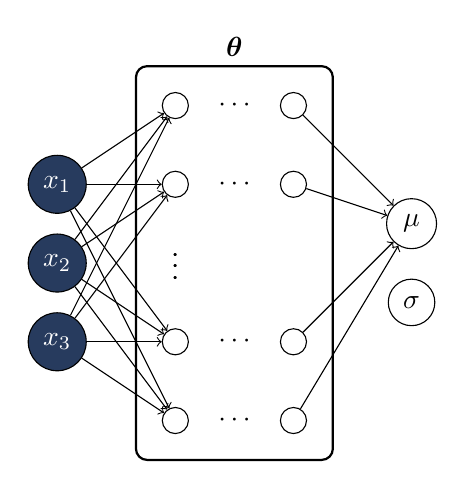
\begin{tikzpicture}
            \pgfmathsetmacro{\firstCol}{0}
            \pgfmathsetmacro{\secondCol}{1.5}
            \pgfmathsetmacro{\thirdCol}{3}
            \pgfmathsetmacro{\fourthCol}{4.5}

            \node[draw, circle, fill=metropolisblue, text=white] (x1) at (\firstCol, 1) {$x_1$};
            \node[draw, circle, fill=metropolisblue, text=white] (x2) at (\firstCol, 0) {$x_2$};
            \node[draw, circle, fill=metropolisblue, text=white] (x3) at (\firstCol, -1) {$x_3$};

            \node[draw, circle, fill=none, text=black] (n11) at (\secondCol, 2) {};
            \node[draw, circle, fill=none, text=black] (n12) at (\secondCol, 1) {};
            \node[draw, circle, fill=none, text=black] (n13) at (\secondCol, -1) {};
            \node[above=0.5cm] at (n13.north) {$\vdots$};
            \node[draw, circle, fill=none, text=black] (n14) at (\secondCol, -2) {};

            % connect all x to all n1 with a for loop
            \foreach \i in {1, 2, 3}
            \foreach \j in {1, 2, 3, 4}
            \draw[->] (x\i) -- (n1\j);

            % create a layer with all horizontal dots
            \foreach \i in {1, 2, 3, 4}
            \node[right=0.25cm] at (n1\i.east) {$\cdots$};

            % create next layer
            \node[draw, circle, fill=none, text=black] (n21) at (\thirdCol, 2) {};
            \node[draw, circle, fill=none, text=black] (n22) at (\thirdCol, 1) {};
            \node[draw, circle, fill=none, text=black] (n23) at (\thirdCol, -1) {};
            \node[above=0.5cm] at (n13.north) {$\vdots$};
            \node[draw, circle, fill=none, text=black] (n24) at (\thirdCol, -2) {};

            % create next layer
            \node[draw, circle, fill=none, text=black] (n31) at (\fourthCol, 0.5) {$\mu$};
            \node[draw, circle, fill=none, text=black] (n32) at (\fourthCol, -0.5) {$\sigma$};

            % connect all n1 to all n2 with a for loop
            \foreach \i in {1, 2, 3, 4}{
                    \draw[->] (n2\i) -- (n31);
                    % \draw[->] (n2\i) -- (n32);
                }

            % draw a rectangle around the first layer and name it \theta
            \draw[rounded corners, thick] (1, 2.5) rectangle (3.5, -2.5);
            \node at (2.25, 2.75) {$\boldsymbol{\theta}$};


        \end{tikzpicture}
        \column{0.4\textwidth}
        \begin{equation*}
            p(y_i| \boldsymbol{x}_i, \boldsymbol{\theta}) = \mathcal{N}(y_i | \mu_i, \sigma^2)
        \end{equation*}
        Find MLE of $\boldsymbol{\theta}$ and $\sigma$ by minimizing the negative log-likelihood

    \end{columns}
\end{frame}

\begin{frame}{Heteroscedastic model with trainable noise}
    % partition page into two columns
    \begin{columns}[T,onlytextwidth]
        \column{0.6\textwidth}
        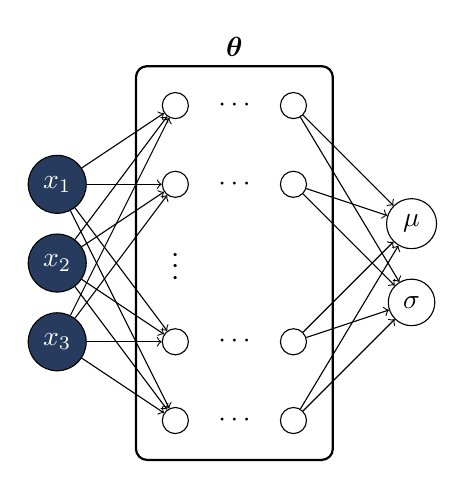
\begin{tikzpicture}
            \pgfmathsetmacro{\firstCol}{0}
            \pgfmathsetmacro{\secondCol}{1.5}
            \pgfmathsetmacro{\thirdCol}{3}
            \pgfmathsetmacro{\fourthCol}{4.5}

            \node[draw, circle, fill=metropolisblue, text=white] (x1) at (\firstCol, 1) {$x_1$};
            \node[draw, circle, fill=metropolisblue, text=white] (x2) at (\firstCol, 0) {$x_2$};
            \node[draw, circle, fill=metropolisblue, text=white] (x3) at (\firstCol, -1) {$x_3$};

            \node[draw, circle, fill=none, text=black] (n11) at (\secondCol, 2) {};
            \node[draw, circle, fill=none, text=black] (n12) at (\secondCol, 1) {};
            \node[draw, circle, fill=none, text=black] (n13) at (\secondCol, -1) {};
            \node[above=0.5cm] at (n13.north) {$\vdots$};
            \node[draw, circle, fill=none, text=black] (n14) at (\secondCol, -2) {};

            % connect all x to all n1 with a for loop
            \foreach \i in {1, 2, 3}
            \foreach \j in {1, 2, 3, 4}
            \draw[->] (x\i) -- (n1\j);

            % create a layer with all horizontal dots
            \foreach \i in {1, 2, 3, 4}
            \node[right=0.25cm] at (n1\i.east) {$\cdots$};

            % create next layer
            \node[draw, circle, fill=none, text=black] (n21) at (\thirdCol, 2) {};
            \node[draw, circle, fill=none, text=black] (n22) at (\thirdCol, 1) {};
            \node[draw, circle, fill=none, text=black] (n23) at (\thirdCol, -1) {};
            \node[above=0.5cm] at (n13.north) {$\vdots$};
            \node[draw, circle, fill=none, text=black] (n24) at (\thirdCol, -2) {};

            % create next layer
            \node[draw, circle, fill=none, text=black] (n31) at (\fourthCol, 0.5) {$\mu$};
            \node[draw, circle, fill=none, text=black] (n32) at (\fourthCol, -0.5) {$\sigma$};

            % connect all n1 to all n2 with a for loop
            \foreach \i in {1, 2, 3, 4}{
                    \draw[->] (n2\i) -- (n31);
                    \draw[->] (n2\i) -- (n32);
                }

            % draw a rectangle around the first layer and name it \theta
            \draw[rounded corners, thick] (1, 2.5) rectangle (3.5, -2.5);
            \node at (2.25, 2.75) {$\boldsymbol{\theta}$};


        \end{tikzpicture}
        \column{0.4\textwidth}
        \begin{equation*}
            p(y_i| \boldsymbol{x}_i, \boldsymbol{\theta}) = \mathcal{N}(y_i | \mu_i, \sigma_i^2)
        \end{equation*}
        Find MLE of $\boldsymbol{\theta}$ by minimizing the negative log-likelihood

    \end{columns}
\end{frame}

\end{document}